
\chapter{多路口场景下交通信号控制}

\section{相关工作}
由于强化学习在单路口交通信号控制上取得了优异的成绩,人们开始致力于使用多智能体强化学习(Multi-Agent Reinforcement Learning, MARL)来解决多路口场景下的交通信号调度。Claus在\inlinecite{claus1998dynamics}中将MARL分为了两类:联合动作学习(Joint Action Learning)和独立学习(Independent Learning)。

对于多路口信号控制,联合动作学习的思想就是使用一个全局智能体(single global agent)来控制所有的交叉路口,其动作是所有路口动作组合在一起的联合动作,然后通过迭代学习建模多个智能体的联合动作价值函数(Joint Action Value Function):
\begin{align}
  Q(o_1, o_2, \cdots, o_N, \mathbf{a})
\end{align}
其中$o_i$是智能体$i$对路口环境的观测,$\mathbf{a}$是所有智能体的联合动作。但是这种方法的缺点是会导致维度灾难(curse of dimensionality),状态动作的联合空间会随着智能体数量的增加呈指数级增长,增加学习的难度。为了缓解这个问题,\inlinecite{van2016coordinated}使用max-plus方法将联合动作价值函数分解为局部子问题的线性组合,如下所示:
\begin{align}
  \hat{Q}\left(o_{1}, \ldots, o_{N}, \mathbf{a}\right)=\Sigma_{i, j} Q_{i, j}\left(o_{i}, o_{j}, \mathbf{a}_{i}, \mathbf{a}_{j}\right)
\end{align}
其中$i \text{和} j$对应于相邻智能体的索引。在\inlinecite{zhang2019integrating,chu2019multi,tan2019cooperative}中,将联合Q值视为局部Q值的加权和:
\begin{align}
  \hat{Q}\left(o_{1}, \ldots, o_{N}, \mathbf{a}\right)=\Sigma_{i, j} w_{i, j} Q_{i, j}\left(o_{i}, o_{j}, \mathbf{a}_{i}, \mathbf{a}_{j}\right)
\end{align}
其中$w_{i,j}$是预先定义的权重。他们试图通过在单个智能体的学习过程的损失函数中增加一个整形项,并使单个Q值的加权和与全局Q值的差异最小化,从而确保单个智能体在学习过程中能够考虑到其他智能体的情况。

多路口信号控制的另一条研究路线是使用独立的RL(IRL)智能体来控制交通信号,其中每个RL智能体控制一个路口。与联合动作学习方法不同,每个智能体可以在不知道其他智能体的奖励信号的情况下学习控制策略。根据智能体之间是否进行信息交互进一步分为以下两类:
\begin{itemize}
  \item IRL without Communication:IRL单独处理每个交叉口,每个agent观察自己的本地环境,不使用显式通信来解决冲突\inlinecite{mannion2016experimental,casas2017deep,zheng2020learning,pham2013learning,liu2018deep,calvo2018heterogeneous,gong2019decentralized}。在一些简单的场景中,如动脉网络,这种方法表现良好,可以形成了几个小绿波(Green waves)。
  然而,当环境变得复杂时,来自相邻agent的非平稳影响将被带到环境中,如果agent之间没有通信或协调机制,学习过程通常无法收敛到平稳策略。为了应对这一挑战,wei在\inlinecite{wei2019presslight}中提出了一个特定的奖励函数,去描述相邻智能体之间的需求从而实现协调。
  
  \item IRL with Communication:这种方法使智能体之间能够就他们的观察进行交流,并作为一个群体而不是个体的集合来完成复杂的任务,在这种情况下,环境是动态的,每个智能体的能力和对世界的可见度是有限的\inlinecite{sukhbaatar2016learning}。
  典型的方法是直接将邻居的交通状况\inlinecite{xu2020network}或过去的动作\inlinecite{ge2019cooperative}加入到自身智能体的观察中,而不是仅仅使用自我观测到的本地交通状况。在这种方法中,不同路口的所有智能体共享一个学习模型,这就需要对相邻的路口进行一致的索引。
  \inlinecite{nishi2018traffic}试图通过利用图卷积网络的路网结构来消除这一要求,以协作附件的多跳路口的交通,并且通过图卷积网络中定义的固定邻接矩阵来模拟相邻代智能体的影响,这表明他们假设相邻智能体之间的影响是静态的。
  在其他工作中,\inlinecite{wei2019colight,wang2020stmarl}提出使用图注意网络来学习相邻智能体和自我智能体的隐藏状态之间的动态相互作用。应该指出的是,利用max-plus学习联合行动学习者的方法和利用图卷积网络学习通信的方法之间有很强的联系,因为它们都可以被看作是学习图上的信息传递,其中前一种方法传递奖励,后一种方法传递状态观测信息。
\end{itemize}

% 目前对于多路口的交通信号调度问题,多数研究工作都是通过使用协作(Coordination)策略来提升路网整体的通行效率,以下列出几种常见的协作策略:
% \begin{table}[htb]
%     \caption[协作策略]{常见的协作策略\label{tab:coordination}}
%     \begin{tabular}{clp{0.4\columnwidth}}
%       \toprule
%       协作策略 & 目标 & 说明 \\
%       \midrule
%       Global single agent & $max_{\mathbf{a}}Q(s, \mathbf{a})$ & $s$是全局的环境状态,$\mathbf{a}$是所有路口的联合动作。\\
%       Independent RL without Communication & $max_{a_{i}}\sum{i}Q_{i}(o_i, a_i)$ & $o_i$是路口$i$的局部观测,$a_i$是路口$i$的动作。\\
%       Independent RL with Communication & $max_{a_i}\sum{i}Q_i(\Omega(o_i, \mathcal{N}_i), a_i)$ &$\mathcal{N}_i$是路口$i$的邻近路口的状态表示,$\Omega(o_i, \mathcal{N}_i)$是整合路口$i$及其邻近路口状态表示的函数。\\
%       \bottomrule
%     \end{tabular}
% \end{table}



\section{已有工作中的不足}
目前大多数工作在使用图神经网络Learn to Communicate的时候,都是以intersection为节点来进行图建模,将每一个路口视作图中的一个节点,每条道路作为连接两个节点的边,很自然地可以将一张交通道路网建模成一个图, 如\autoref{fig:network-graph-old}所示:
\begin{figure}[htb]
  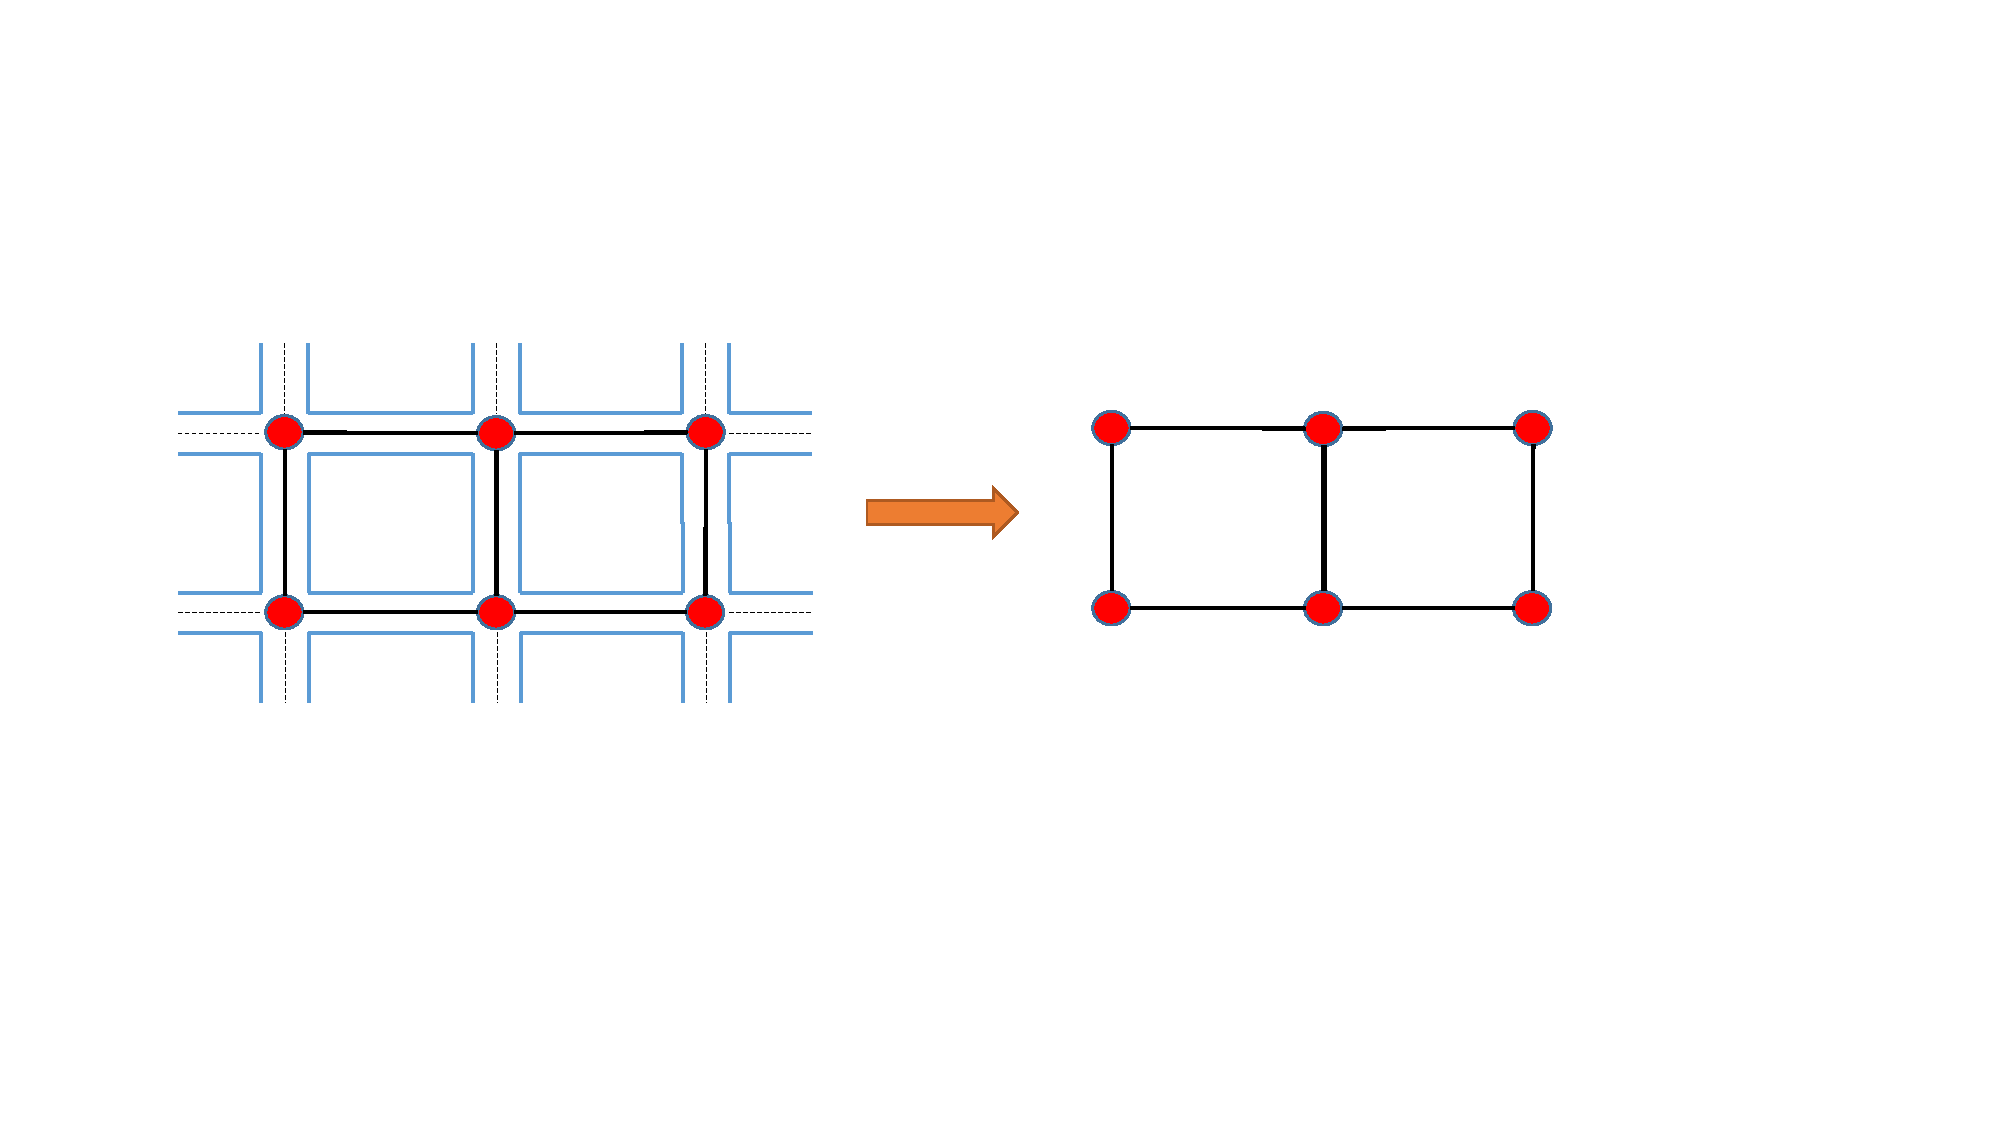
\includegraphics[width=0.9\textwidth]{ppt/network-graph.pdf}
  \caption{多路口建模成图(路口)}
  \label{fig:network-graph-old}
\end{figure}
在这种建模方式下,每条车道的车辆以及当前的相位将作为该节点的特征。这种建模方式虽然可以很清晰的将多路口场景变成一张图。但是,因为是以一个路口为一个节点,所有车道的状态信息都整合到了一起,有些车道的的信息对目标节点是无用的,
如\autoref{fig:information-redundancy}所示:
\begin{figure}[htb]
  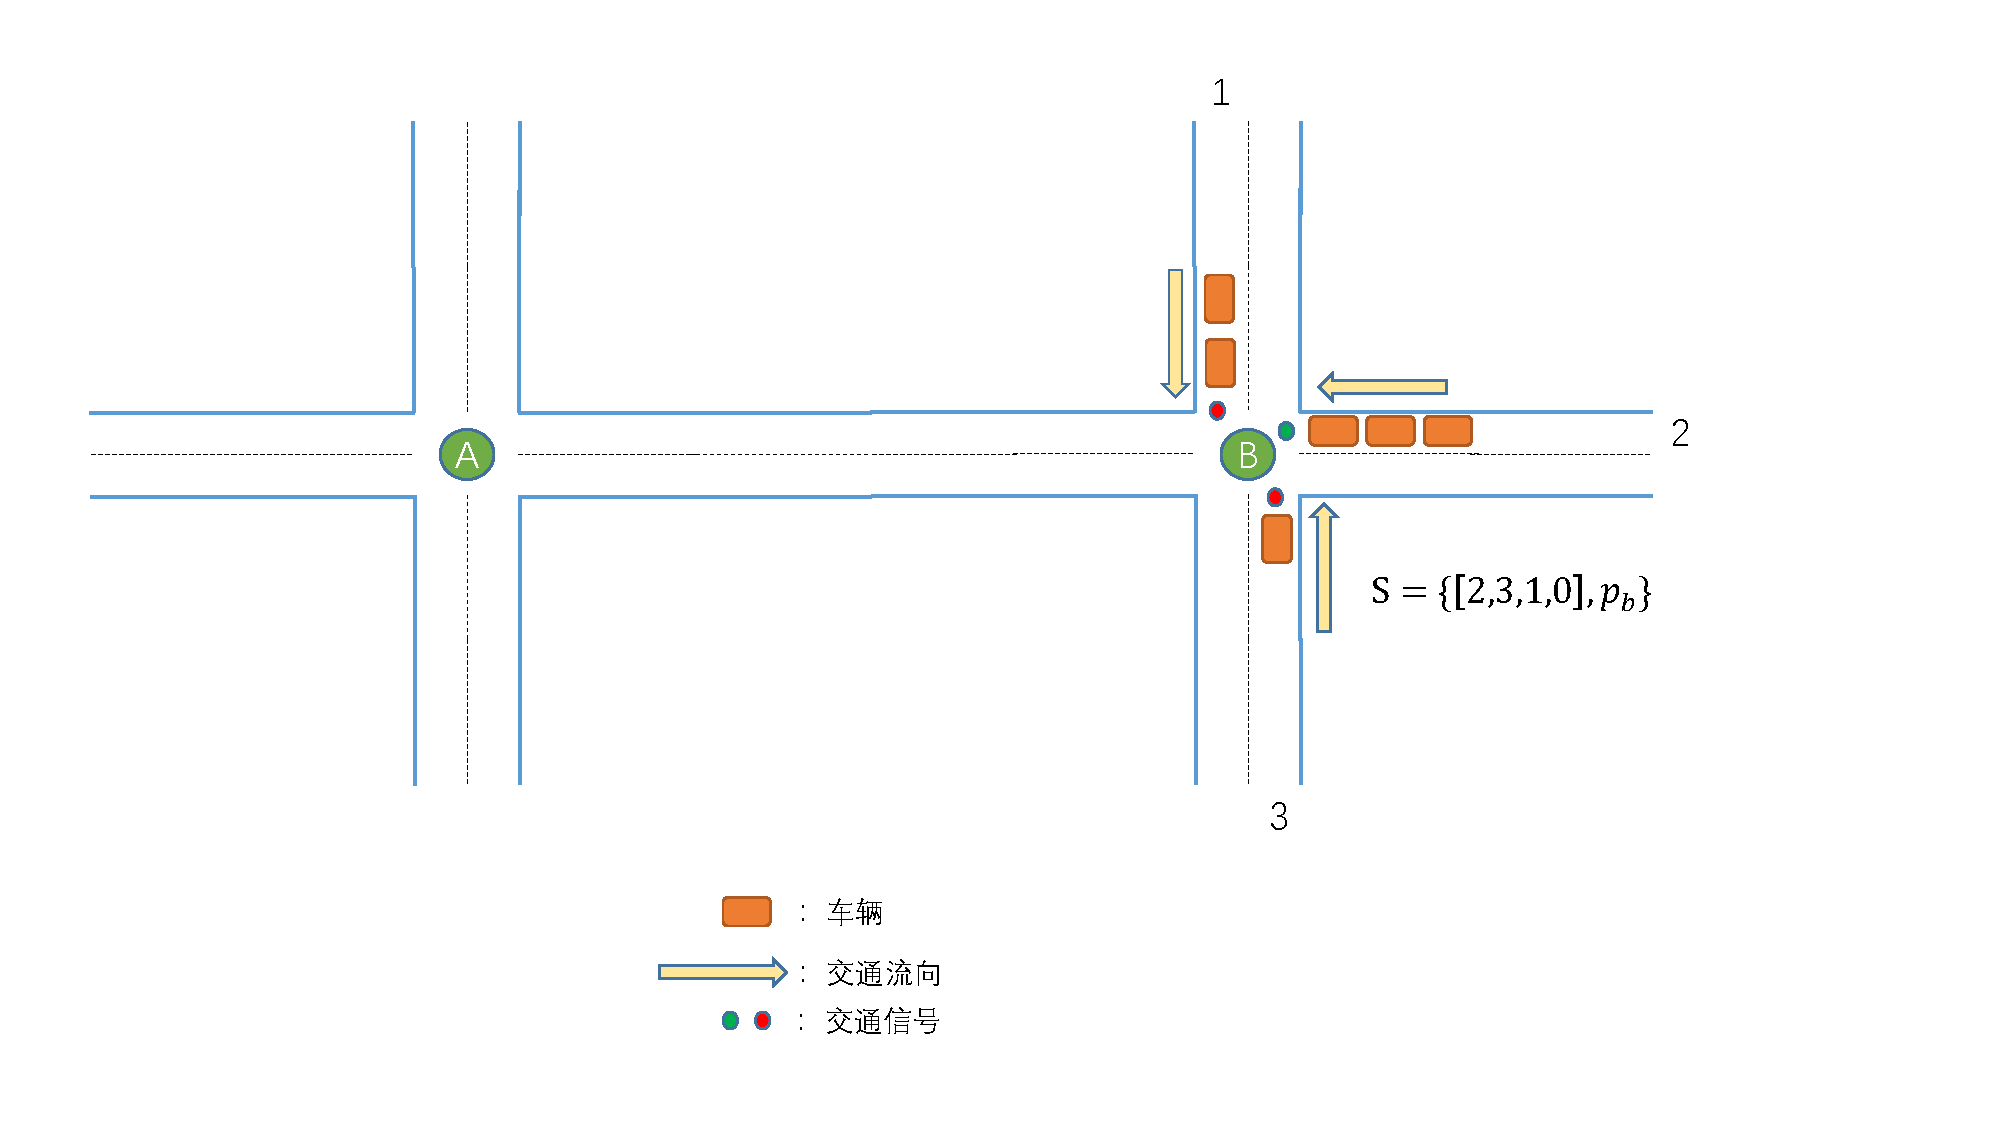
\includegraphics[width=0.9\textwidth]{ppt/information-redundancy.pdf}
  \caption{按路口建图模式下信息传递}
  \label{fig:information-redundancy}
\end{figure}
路口B中只有2车道的交通流向与A车道有关,1、3车道的车辆不会行驶到A路口。在信息传递的时候,如果将所有的信息都笼统地传递过去,将会增加A提取有效信息的难度,从而降低学习的效率。

\section{改进}
本文同样采用IRL with Communication的框架,与已有工作不同的是,我们采用不同的建模方式:以道路为节点进行图建模,即一条道路就是一个节点,如\autoref{fig:network-graph-new}所示:
\begin{figure}[htb]
  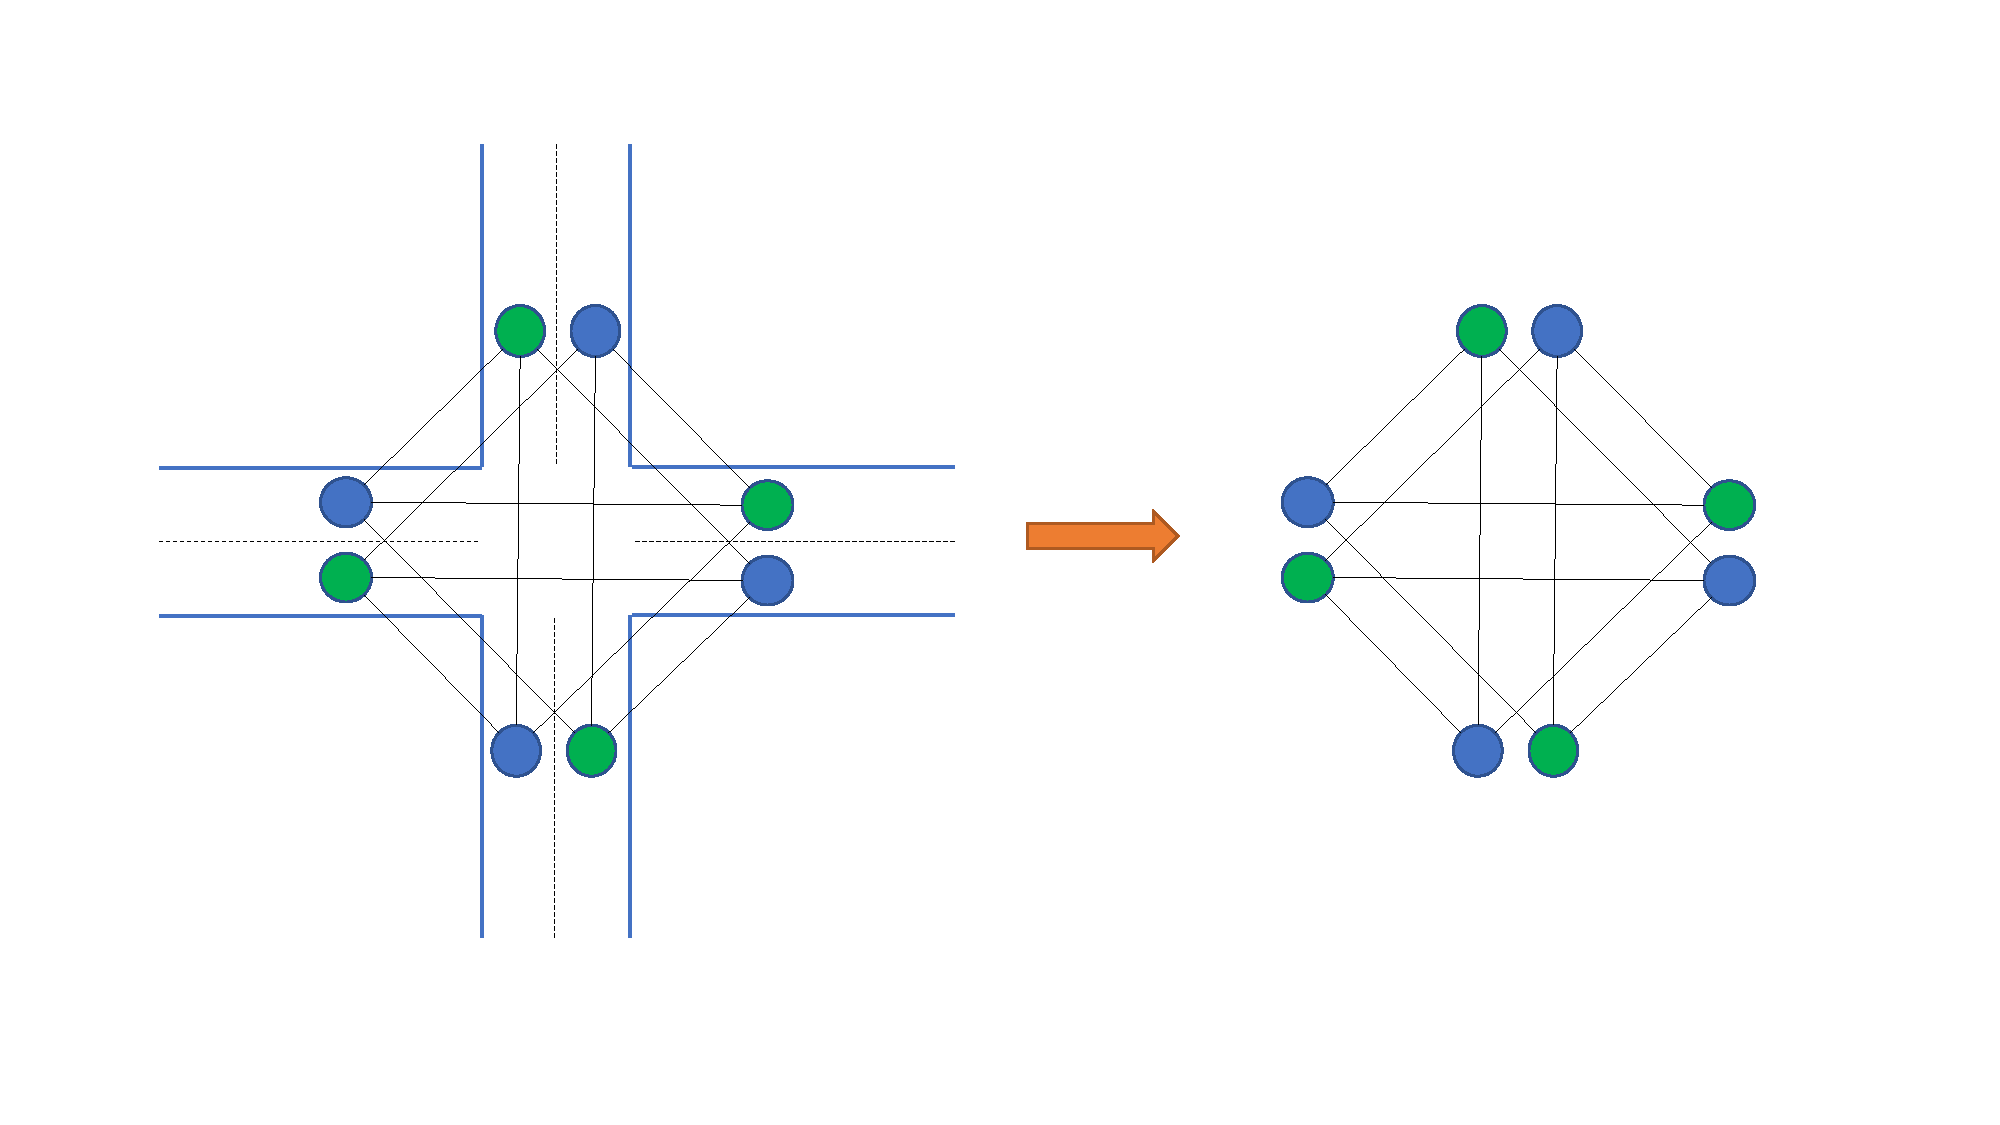
\includegraphics[width=0.9\textwidth]{ppt/graph-modeling.pdf}
  \caption{按道路建模成图}
  \label{fig:network-graph-new}
\end{figure}

此外,我们根据当前的相位对图的边设一个权重。这里我们规定,如果在当前相位下,道路$i$到道路$j$之间的交通是允许通行的,则表示$(i,j)$的状态是'connected'。权重的定义方法如下:
\begin{align}
  w_{i,j} = \begin{cases}
    1 & (i, j) \text{ is connected} \\
    0 & \text{otherwise}
  \end{cases}
\end{align}
这个权重将被用于剔除对目标节点无用的信息。

这里我们沿用\inlinecite{wei2019colight,wang2020stmarl}工作使用图注意网络,但是与之不同的是,我们不是学习相邻智能体和目标智能体的隐藏状态之间的动态相互作用,而是用来估计目标智能体在下一个时间节点的交通状态。
\section{方法}
整个过程可以分解为以下几个步骤:

\section{实验}

